%%%%%%%%%%%%%%%%%%%%%%%%%%%%%%%hhhhhh%%%%%%%%%
% APA Assignment Article
% LaTeX Template
% Version 2.0 (February 7, 2023)
%
% This template originates from:
% https://www.LaTeXTemplates.com
%
% Author:
% Vel (vel@latextemplates.com)
%
% License:
% CC BY-NC-SA 4.0 (https://creativecommons.org/licenses/by-nc-sa/4.0/)
%
% NOTE: The bibliography needs to be compiled using the biber engine.
%
%%%%%%%%%%%%%%%%%%%%%%%%%%%%%%%%%%%%%%%%%

%----------------------------------------------------------------------------------------
%	PACKAGES AND OTHER DOCUMENT CONFIGURATIONS
%----------------------------------------------------------------------------------------

\documentclass[
	letterpaper, % Paper size, use either a4paper or letterpaper
	10pt, % Default font size, can also use 11pt or 12pt, although this is not recommended
	unnumberedsections, % Comment to enable section numbering
	twoside, % Two side traditional mode where headers and footers change between odd and even pages, comment this option to make them fixed
]{APAAssignment}

\addbibresource{bibliography.bib} % BibLaTeX bibliography file

\runninghead{MICS CYBER 252, Fall-2024 Hands On Lab Unit 13} % A shortened article title to appear in the running head, leave this command empty for no running head

\footertext{\textit{Hands On Lab 13} (MICS CYBER 252, Fall -2024)} % Text to appear in the footer, leave this command empty for no footer text

\setcounter{page}{1} % The page number of the first page, set this to a higher number if the article is to be part of an issue or larger work

%----------------------------------------------------------------------------------------
%	TITLE SECTION
%----------------------------------------------------------------------------------------

\usepackage[title,toc,titletoc]{appendix}
\usepackage{titlesec}
\usepackage{lscape}
\usepackage{fontawesome}

\title{Hands On Lab: Unit 13 \\ MICS-252, Fall 2024 \\ Digital Forensics II \\ Image Analysis}

% Authors are listed in a comma-separated list with superscript numbers indicating affiliations
% \thanks{} is used for any text that should be placed in a footnote on the first page, such as the corresponding author's email, journal acceptance dates, a copyright/license notice, keywords, etc
% Affiliations are output in the \date{} command
\date{UC Berkeley School of Information \\
MICS Course 252 Fall 2024 (Kristy Westphal)
}


\author{
	Prepared by: Karl-Johan Westhoff \\
	email: \href{mailto:kjwesthoff@berkeley.edu}{kjwesthoff@berkeley.edu}
}


% % Full-width abstract
% \renewcommand{\maketitlehookd}{%
% 	\begin{abstract}
% 		\noindent Lorem ipsum dolor sit amet,rta porttitor.
% 	\end{abstract}
% }

%----------------------------------------------------------------------------------------

\setcounter{tocdepth}{5}
\setcounter{secnumdepth}{5}
\usepackage[title]{appendix}

\begin{document}
\onecolumn
\maketitle % Output the title section

%----------------------------------------------------------------------------------------
%	ARTICLE CONTENTS
%----------------------------------------------------------------------------------------

\section{Introduction}
We are given an Encase .E01 image: "Windows Image.E01" with a size of 10.6 GB. The image was ingested into Autopsy version 4.21. We are given the following objectives for the exercise, to get thoroughly around the disc image.

\subsection{Objectives}

Attempt to answer the following questions:
\begin{itemize}
	\item What time zone is the image set in?
	\item What Operating System is the suspect drive using?
	\item What event happened on January 1, 1980?
	\item What is the IP address of the suspect drive?
	\item What is the EvenMoreSecretStuff.vhd (and can you see what is in it?)
	\item Do any of the suspicious items discovered look suspicious to you?
	\item Anything else that you found that you want to highlight?
\end{itemize}

\subsection{Autopsy report}
Autopsy has functionality to generate a report of the findings in various formats. I have published the report on github pages for reference in this report as:
\begin{itemize}
	\item	\cite{AutoReport}: \url{https://kjwesthoff.github.io/252-Lab13-AutopsyReport/}
\end{itemize}


\section{Image Ingestion}
The file name indicates that the file is a Windows pc image. Anyway, the image was subjected to the full slew on ingest modules from the default Autopsy 4.21 installation (See Case Summary section of \cite{AutoReport}). The execution of various ingestion modules was a lengthy process (>24hrs. in this case). Autopsy can include custom ingestion modules that analyse the file hashes against known malware, in this case hashes were generated for all files (hence the lengthy ingest) and are thus ready for comparison against a database of known hashes (considered out of scope for this assignment), luckily most of Autopsy's functionality is available while it analyzes the files, and various result sections are populated as they become available.

\section{Analysis Results}
The Image holds two data sources; Windows Image.E01 and EvenMoreSecretStuff.vhd, the .vhd extension indicates that it is a Windows Virtual Hard Disc \cite{WindowsVHD}
\subsection{Assignment Objectives Results}

\subsubsection{Time Zone}
Both data sources indicate: "America/Los Angeles", and the images were acquired on Mar. 20, 2019 in the evening around 8pm, see Appendix \ref{app:MetaData}

\subsubsection{Operating System}
Both the .E01 file name, the .vhd part and various artifacts indicate a Windows OS, the Autopsy report \cite{AutoReport} indicated:

\begin{itemize}
	\item OS: "Windows 10 Enterprise"
	\item product ID "00329-00000-00003-AA856"
	\item built for: "AMD64 architecture"
	\item with the business like computer name: "DESKTOP-0QT8017"
\end{itemize}

\subsubsection{Event on January 1, 1980:}
January 1 1980 at midnight is the epoch (beginning of time) for MS-DOS\footnote{I was about to write that it was when "Skynet became self-aware" but that was August 29, 1997 \cite{enwiki:Terminator}}. For unix systems it is January 1. 1970 (of course Microsoft had to have their own epoch). When computers get confused or are missing a time stamp they default to epoch. In this case it is apparently some google chrome files that is causing some confusion, see Appendix \ref{app:Jan1980}


%
%\begin{figure}[!h] % Single column :figure	
%	\centering
%	\includegraphics[width=1\linewidth]{Autopsy4_2:w1.png}
%	\caption{Autopsy version 4.21, installed desktop application}
%	\label{fig:Autopsy4_21}
%\end{figure}
%










\section{Conclusion}

\clearpage
\printbibliography % Output the bibliography   

%----------------------------------------------------------------------------------------



%----------------------------------------------------------------------------------------
%	 Appendices
%----------------------------------------------------------------------------------------
%
%\appendix


\clearpage
\chapter{Appendices}
\begin{appendices}

	\section{Image MetaData}\label{app:MetaData}


	\begin{figure}[!h] % Single column :figure	
		\centering
		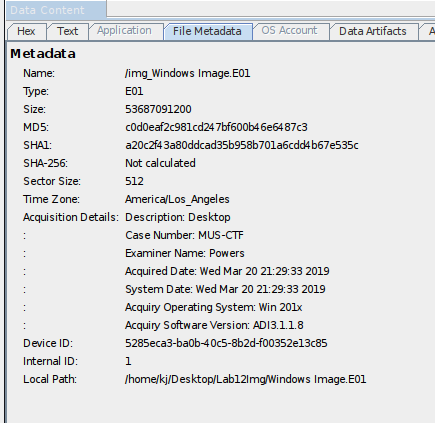
\includegraphics[width=0.5\linewidth]{WindowsImageMetadata.png}
		\caption{Meta data for the Windows image.E01 Data source}
		\label{fig:windowsIageMetadata}
	\end{figure}


	\begin{figure}[!h] % Single column :figure	
		\centering
		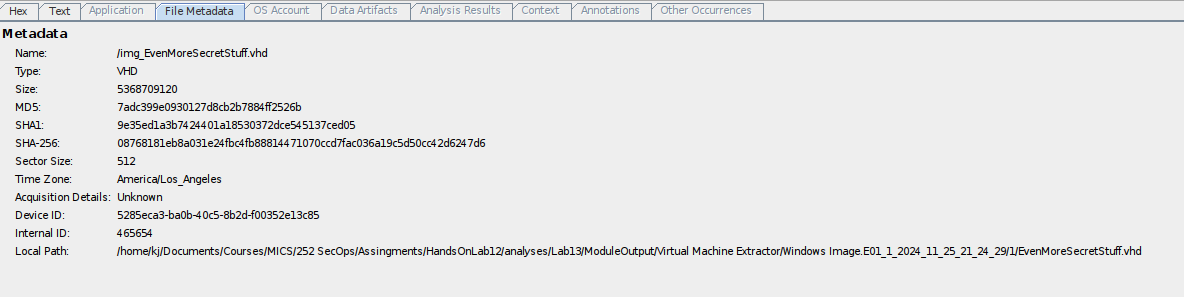
\includegraphics[width=1\linewidth]{MoresecretStuffMetadata.png}
		\caption{Meta data for the "EvenMoreSecretStuff" Data source}
		\label{fig:evenMoreSecretStuffMetaData}
	\end{figure}
	\clearpage
	\section{January 1. 1980}\label{app:Jan1980}


	\begin{figure}[!h] % Single column :figure	
		\centering
		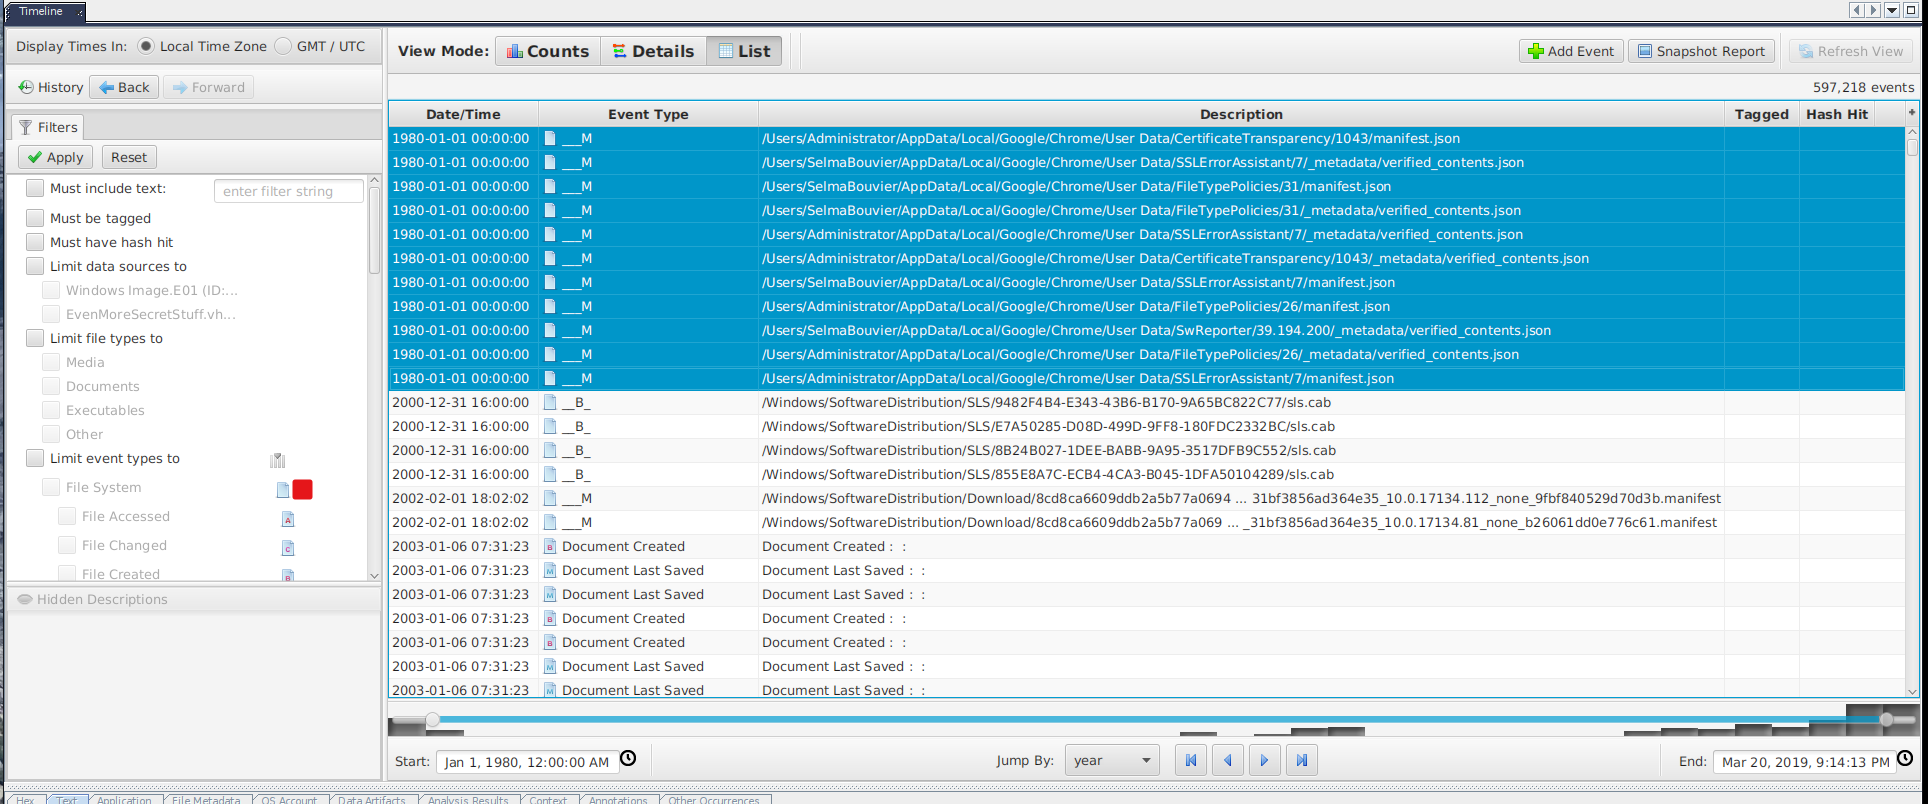
\includegraphics[width=1\linewidth]{Jan1980.png}
		\caption{Timeline results for January 1. 1980}
		\label{fig:Jan1980}
	\end{figure}



\end{appendices}




\end{document}
